\chapter{Architecture}\label{ch:architecture}

\begin{figure}[h]
    \centering
    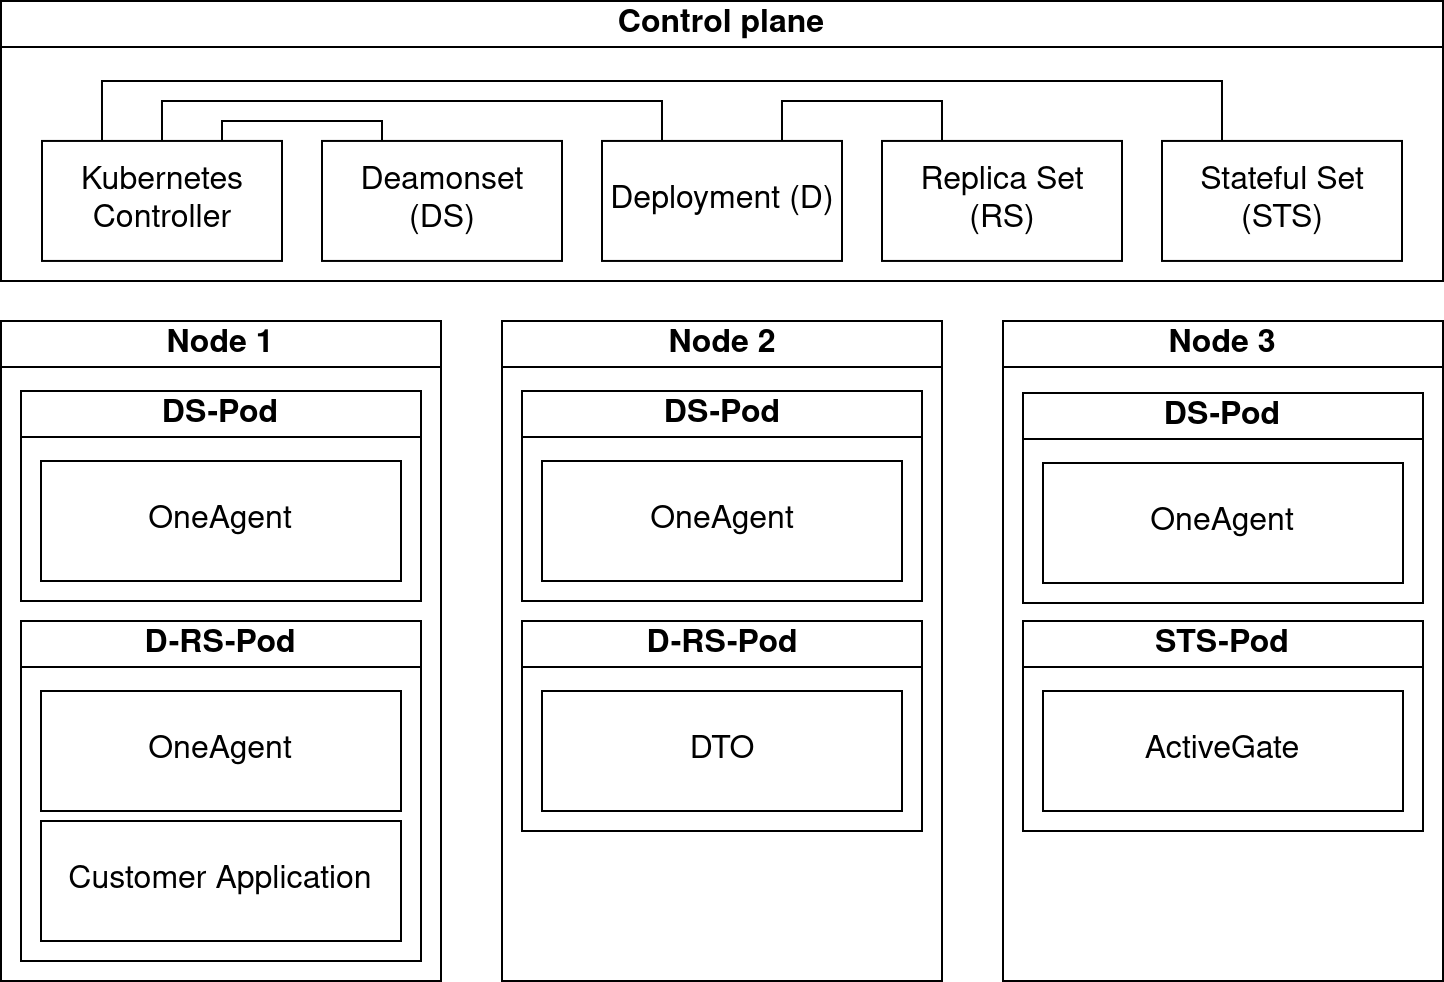
\includegraphics[width=\textwidth]{img/context/kubernetes}
    \caption{Kubernetes architecture.}
    \label{fig:kubernetes-architecture}
\end{figure}

In Figure~\ref{fig:kubernetes-architecture}, an exemplary setup of all the previously discussed technologies can be seen.
The Kubernetes controller is aware of all its resources.
In this example, the relevant resources are deamonsets, deployments and the replicasets they control, and stateful sets.
If the DTO is configured as such, it deploys OneAgents monitoring the host, using a daemonset, so they are deployed once on every node.
Then it creates a statfulset which deploys an instance of an ActiveGate.
Finally, the webhook of the DTO injects scheduled customer pods with application specific OneAgents.

This setup is one of the simplest setups that is possible while still being representative of real world example.
It becomes apparent why a complex test setup is needed, since the environment the DTO runs in is equally complex.
A Kubernetes cluster must be created and setup for it to run in.
Example applications must be deployed and configured for correct injection.

\begin{figure}[H]
    \centering
    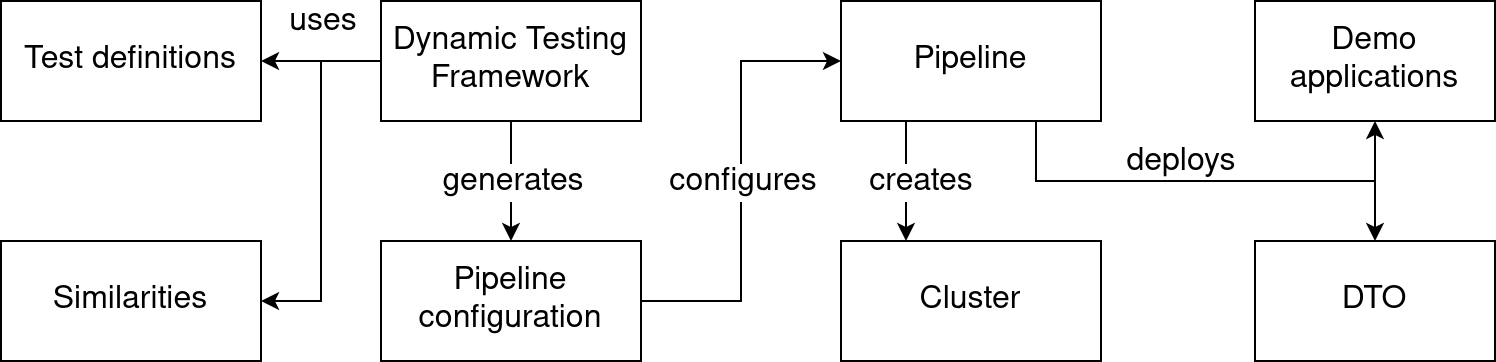
\includegraphics[width=\textwidth]{img/context/dtf}
    \caption{Dynamic Testing Framework workflow.}
    \label{fig:dtf-workflow}
\end{figure}

In Figure~\ref{fig:dtf-workflow} the general workflow of the DTF is shown.
Test definitions and how similarities are used are explained in Section~\ref{subsec:test-definitions} and Section~\ref{subsec:similarities}.
The DTF uses both to generate a pipeline configuration for Concourse.
This configuration can then be applied to a running Concourse instance and started.

The idea is, that this pipeline then creates a cluster, configures it and deploys the DTO as well as needed applications on it.
Further tasks of this pipeline can then check for specific states when applying different DTO configurations.
After all tests succeeded, a second pipeline, the release pipeline, can be triggered.

\begin{figure}[H]
    \centering
    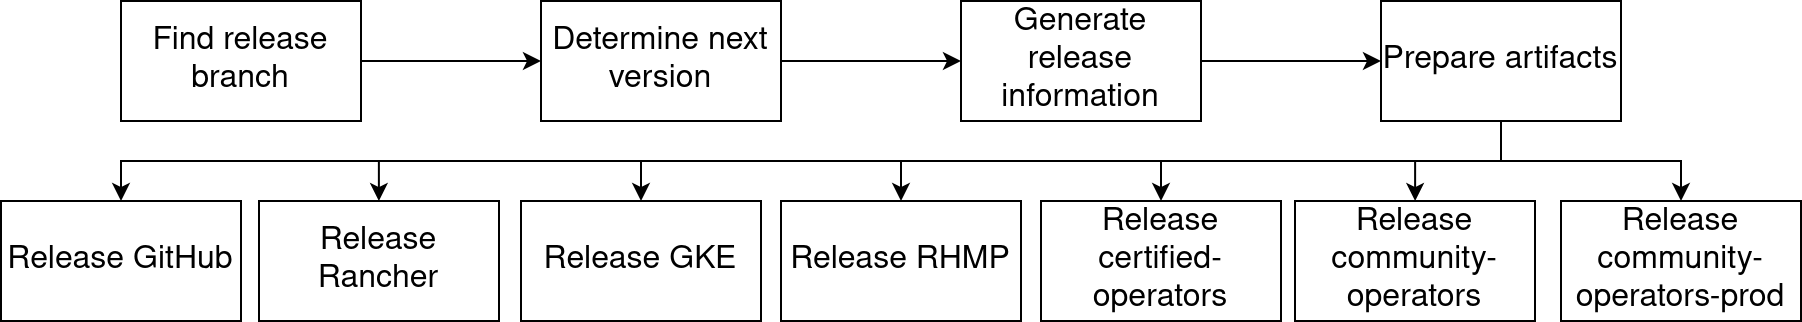
\includegraphics[width=\textwidth]{img/context/release pipeline}
    \caption{Release pipeline.}
    \label{fig:release-pipeline}
\end{figure}

\pagebreak

The general principle behind the release pipeline is depicted in Figure~\ref{fig:release-pipeline}.
First, it is assumed that there is a single source of truth.
This source is the repository in which the DTO's code and other development files reside.
From this repository, the next release that is supposed to happen is determined.
Using the files or information in this release branch the next version can be inferred.
The contents of the repository can then be combined with the version information and release information can be generated.
Afterwards, all necessary artifacts, such as binaries, images and Helm charts, can be compiled, built and generated.
Finally, the releases to the specific marketplaces are triggered.
These tasks can run in parallel and execute the steps that are specific to each marketplace.
